\documentclass[12pt,oneside,a4paper]{hepthesis}

% Language-Encoding und Font
\usepackage{polyglossia}        % Alternative zu Babel
\setmainlanguage[babelshorthands=true]{german}
\setotherlanguage[variant=british]{english}
\addtokomafont{labelinglabel}{\sffamily} % ???
\usepackage{fontspec}           %
\usepackage{unicode-math}
% \setmainfont{Times New Roman}   % Unverhältnismäßig hässlich. Besser keine Font
                                % setzen.

% Formatierung
\usepackage{geometry}           % Paket für Änderung der Seitenränder
\usepackage{setspace}           % Paket für Zeilenabstand
\spacing{1.25}                  % Zeilenabstand setzen
\geometry{a4paper,left=20mm,right=20mm, top=20mm, bottom=20mm, headsep=7mm}
\raggedbottom{}
\usepackage{microtype}

% Citation, Verweise
\usepackage{harvard}
\usepackage{nameref}
\usepackage{glossaries}         % \gls{<golssary-entry>} makeglossaries <dateiname> per cmd
\usepackage{listings}           % Paket zum Einfügen von Source Code.
                                % REPLACE https://tex.stackexchange.com/questions/102596/minted-vs-texments-vs-verbments/103471#103471:

% Fileinsertion
\usepackage{pdfpages}           % Paket zum Einfügen von PDFs
\usepackage{hyperref}[]         % Einträge im Inhaltsverzeichnis werden zu Links,
                                % muss das letzte Package sein
% Tabellen etc
\KOMAoption{numbers}{noenddot}  % Keine End-Punkte (4., 4.1.) in Nummerierungen???
\usepackage{booktabs}           % Tabellenpaket, Keine vertikal und dicken Linien

% Sonstiges
\usepackage{ulem}               % Unterstreichen von Text
\usepackage{titling}  
\usepackage[german]{datetime2}  % Gerade gar nicht genutzt?!
\usepackage{blindtext}          % Repräsentativer als Lorem Ipsum
\usepackage{todonotes}          % Einfügen von Todos

%%%% <Workarounds> %%%%
% Für Package:todonotes
\setlength{\marginparwidth}{2cm}

% Fix für unbekannten Fehler
\DeclareOldFontCommand{\bf}{\normalfont\bfseries}{\mathbf}

% stoppt Floats an Section-Grenzen
\usepackage[section]{placeins}

% Fügt \FloatBarrier an subsections. Hält Floats davon ab, zu verrutschen.
\makeatletter
\AtBeginDocument{%
  \expandafter\renewcommand\expandafter\subsection\expandafter{%
  \expandafter\@fb@secFB\subsection{}
  }%
}
\makeatother

% Math-Bugfixes
\usepackage{lualatex-math}

%%%% </Workarounds> %%%%


\makeglossaries{}

% Metadaten %
\title{Stempelerkennung in Antragsformularen durch Machine Learning}
\author{8323}
\date{\today}
\hypersetup{
 pdfauthor = {\theauthor},
 pdftitle = {\thetitle},
 pdfsubject = {Transferleistung, Techniker Krankenkasse/Nordakademie, 2018},
 bookmarksopen=true
}


% Eigene Variablen und Commands %
\newcommand{\theLocationAndDate}{Hamburg, den \thedate}


\begin{document}

%\setacronymstyle{long-short-desc}

% ----------------------------- Acronyms -----------------------------
\newacronym[description={Organisation von
Workinggroups, die sich mit je einem spezifischen Thema befassen. Teil der
Internet Society (ISOC)}]{ietf}{IETF}{Internet Engineering Task Force}
\newacronym[description={hostet Nutzerinformationen}]{idp}{IdP}{Identity
Provider}
\newacronym[description={Umsetzung eines Features oder Produktes mit zwar
minimalem Funktionsumfang, aber dennoch konkretem Mehrwert für den Nutzer},
plural={MVPs}] {mvp}{MVP}{Minimal Viable Product}
\newacronym[description={Protokoll zur hybriden Verschlüsselung von
Datenübertragungen, Grundlage für HTTPS}]{TLS}{TLS}{Transport Layer Security}

% ----------------------------- Glossary Entries -----------------------------

\newglossaryentry{OAuth} {
    name={OAuth 2.0},
    description={Protokoll zur API-basierten Autorisierung}
}
\newglossaryentry{RO} {
    name={Resource Owner},
    description={Im \gls{OAuth}-Kontext, Besitzer einer oder mehrer Ressourcen, auf die eine andere Anwendung Zugriff erhalten möchte.}
}
\newglossaryentry{Grant Type} {
    name={Grant Type},
    plural={Grant Types},
    description={bestimmt, wie Clients Authorization Grants von Resource Ownern
    erhalten können. Die vier Grant Types\: Authorization Code, Implicit, Resource Owner Password Credentials sowie Client Credentials wurden in RFC 6749
    definiert; auch eigene Grant Types zu definieren ist möglich~\citevgl[S.~23ff.]{RFC6749}}.
}

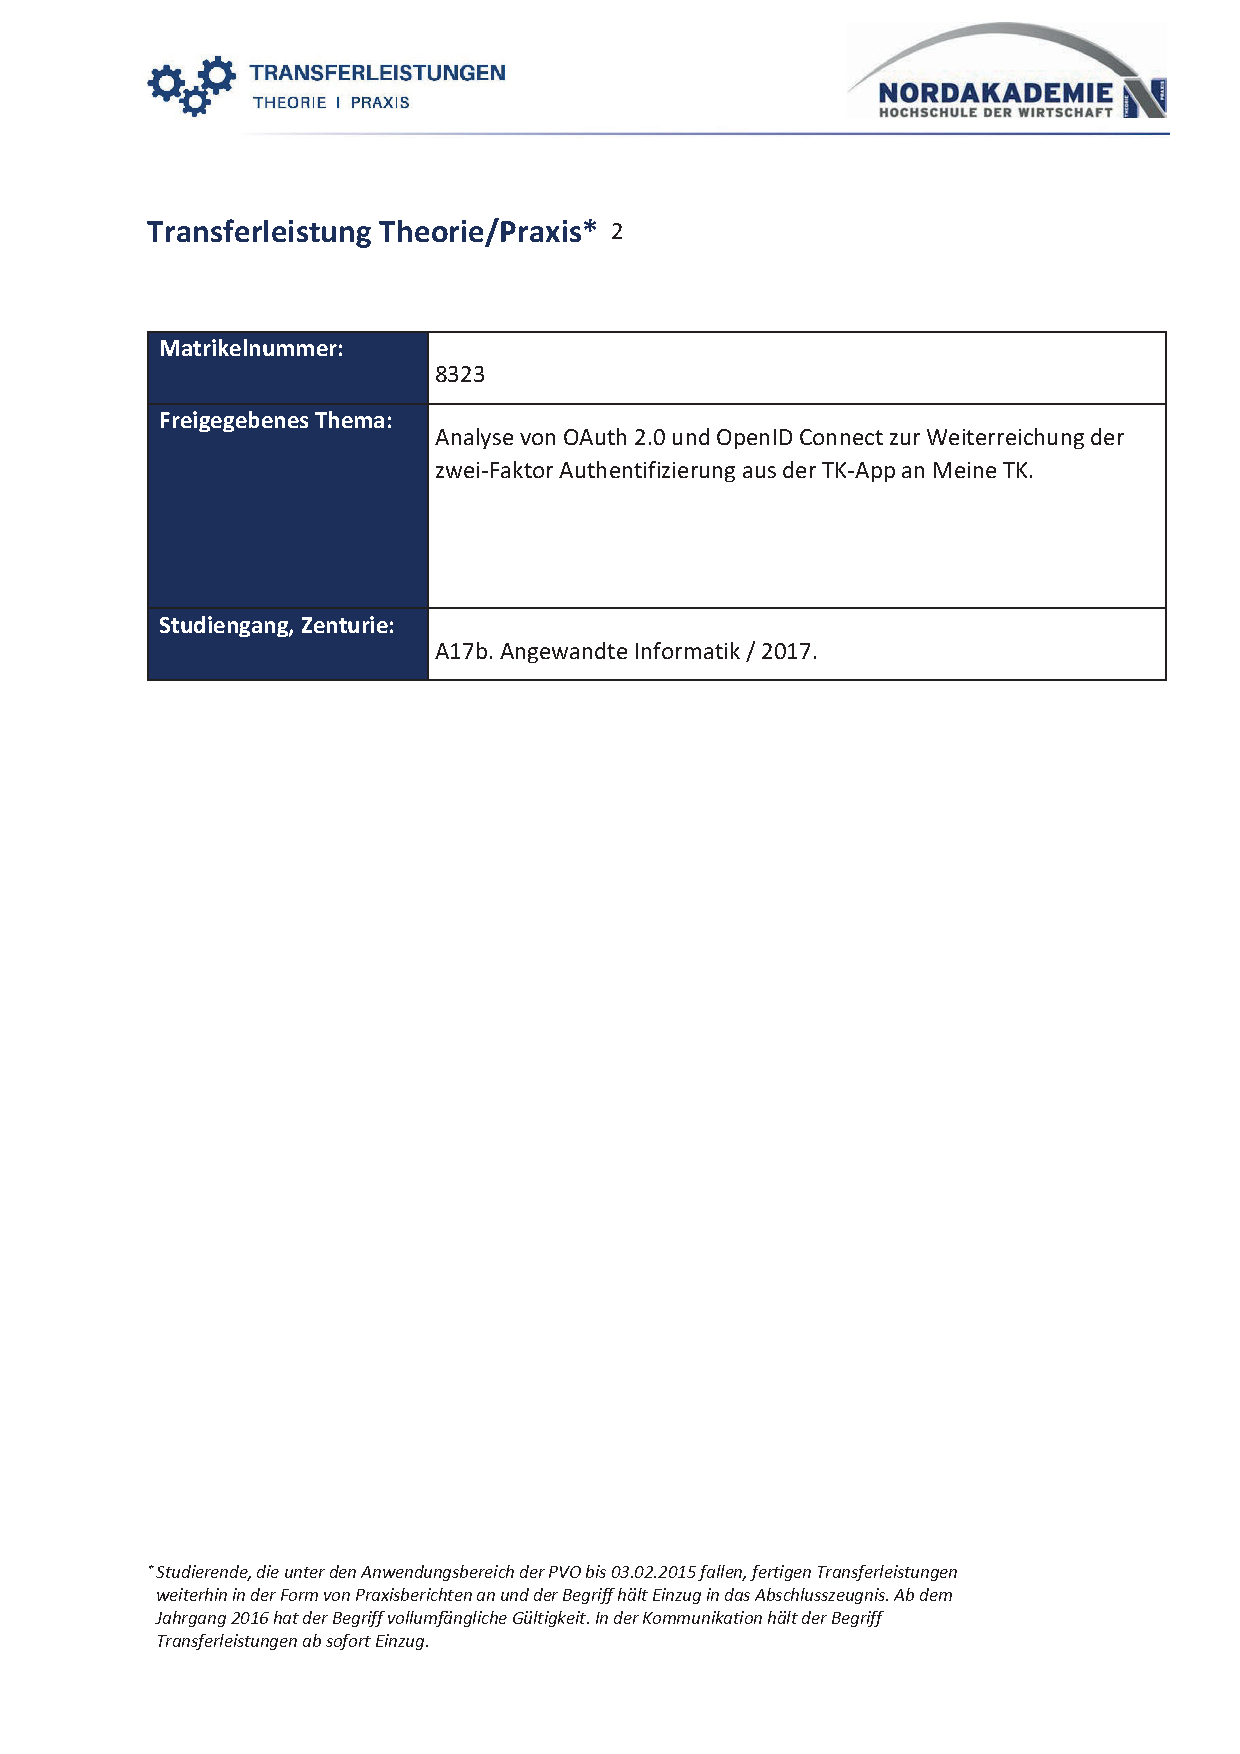
\includepdf[pages=1]{misc/deckblattTerminiert.pdf}
\newpage


\begin{frontmatter}
% Enthält:
  % Klassische Titelseite
\thispagestyle{empty}
\begin{center}
\vspace*{-2cm}
\includegraphics[width=0.85\textwidth]{\detokenize{Logo_NAK}}\\
\vspace*{1.5cm}
    {\titlefont\huge\onehalfspacing{}
	\thetitle{}
    \par}%
\vfill
{
\vspace*{1.5cm}
    \normalfont\normalcolor\bfseries\large
    Transferleistung \\
    \large
    im Studiengang Angewandte Informatik\\
    angefertigt im Projekt-Team Künstliche Intelligenz\\
    der Techniker Krankenkasse\\
    \par
}
\noindent \textbf{Martrikelnummer: \theauthor}\\
\end{center}\par
%\vfill
%\vspace*{2.5cm}
\noindent\begin{minipage}[b]{\textwidth}
{
%\noindent \textbf{von \theauthor, geb.~am 01.~März 1998 in Bad Oldesloe}\\

%  \begin{tabbing}
  %  \textbf{Betreuer und Prüfer:}  \= \textbf{Jan Koops, Tech-Lead TK-App}
  %\textbf{2. Betreuer und Prüfer:}  \= \textbf{Philip MacDonald, Full-Stack/IOS}\\
  %\textbf{3. Betreuer und Prüfer:}  \= \textbf{Jan Ove Weichel, Android}\\
%  \end{tabbing}
  \vspace*{5cm}
  \noindent\textbf{\theLocationAndDate}
}
\end{minipage}

  \begin{abstract}[Abstract]
    \thispagestyle{plain} \addtocounter{page}{-1} \fussy
    \blindtext{}
\end{abstract}
  \tableofcontents \newpage \thispagestyle{empty}
  Hello World

  Hello World
  Hello World ÄÖÜüäöß
  Hello World

  \subsection*{Sperrvermerk}
\thispagestyle{empty} \addtocounter{page}{-1}
Die Inhalte dieser Arbeit betreffen Informationen über betriebliche Belange der
Techniker Krankenkasse. Dies gilt ebenfalls bezüglich der für die Beurteilung
der Arbeit zur Verfügung gestellten Dokumente der Techniker Krankenkasse. Die
Arbeit selbst und weitere Dokumente sind für den innerbetrieblichen Gebrauch
bestimmt und dürfen somit der Öffentlichkeit – auch in Auszügen – nicht
zugänglich gemacht werden.
  \newpage
  \thispagestyle{empty}
  \addtocounter{page}{-3}
\end{frontmatter}

\begin{mainmatter}
  \blindtext[5]
  %\chapter{Einleitung} Seit ungefähr 2016 erprobt die TK Softwareentwicklung in
agilen Teams. Das Team Online and Mobile Projects, in dem diese Arbeit entstand,
ist eines der Pilotprojekte dieses Vorstoßes. Das Team ist unter anderem mit der
Betreuung und Weiterentwicklung der TK-App betraut. Die TK-App versucht,
Verwaltungsprozesse, Kundeninteraktion im Allgemeinen, nutzerfreundlich
umzusetzen.\\ In Meine TK, der Web-Plattform für Versicherte der TK, sind einige
der von uns für die App geplanten Prozesse bereits vorhanden. Teil der agilen
Planung ist das \gls{mvp}. \glspl{mvp} sind minimal nutzbare Produkte. Im Rahmen
eines  \gls{mvp}s ist es denkbar, einen Prozess im ersten Schritt nur teilweise
in der App zu verwirklichen, den Nutzer ab einem bestimmten Punkt an Meine TK
weiterzuleiten und den Prozess dort fortzusetzen. Hierzu müssen Nutzer sich
derzeit stets erneut einloggen. Ziel dieser Arbeit ist, den Prozess der
Weiterleitung für Nutzer angenehmer zu gestalten, indem die erneute Eingabe
seiner Daten für ihn entfällt.\\ Die Weiterleitung von Zugriffsrechten ist seit
2012 mit der Veröffentlichung von \gls{OAuth}
\textit{grundsätzlich} keine schwere Aufgabe mehr. Da die TK jedoch hohe
Ansprüche an ihrer Sicherheitsstandards stellt und die Sicherheit der
Implementierung eines Protokolls nicht durch die Sicherheit des Protokolls
sichergestellt ist, wie~\cite{Sun.2012,Hu.2014,Yang.2016} zeigten, ist diese
Arbeit entstanden.\\ Die Frage, ob sich OAuth, das als Autorisierungsverfahren
gedacht ist, für die Authentifizierung eines Nutzers eignet, wird in dieser
Arbeit elegant umschifft.

  %\chapter{Einleitung} Seit ungefähr 2016 erprobt die TK Softwareentwicklung in
agilen Teams. Das Team Online and Mobile Projects, in dem diese Arbeit entstand,
ist eines der Pilotprojekte dieses Vorstoßes. Das Team ist unter anderem mit der
Betreuung und Weiterentwicklung der TK-App betraut. Die TK-App versucht,
Verwaltungsprozesse, Kundeninteraktion im Allgemeinen, nutzerfreundlich
umzusetzen.\\ In Meine TK, der Web-Plattform für Versicherte der TK, sind einige
der von uns für die App geplanten Prozesse bereits vorhanden. Teil der agilen
Planung ist das \gls{mvp}. \glspl{mvp} sind minimal nutzbare Produkte. Im Rahmen
eines  \gls{mvp}s ist es denkbar, einen Prozess im ersten Schritt nur teilweise
in der App zu verwirklichen, den Nutzer ab einem bestimmten Punkt an Meine TK
weiterzuleiten und den Prozess dort fortzusetzen. Hierzu müssen Nutzer sich
derzeit stets erneut einloggen. Ziel dieser Arbeit ist, den Prozess der
Weiterleitung für Nutzer angenehmer zu gestalten, indem die erneute Eingabe
seiner Daten für ihn entfällt.\\ Die Weiterleitung von Zugriffsrechten ist seit
2012 mit der Veröffentlichung von \gls{OAuth}
\textit{grundsätzlich} keine schwere Aufgabe mehr. Da die TK jedoch hohe
Ansprüche an ihrer Sicherheitsstandards stellt und die Sicherheit der
Implementierung eines Protokolls nicht durch die Sicherheit des Protokolls
sichergestellt ist, wie~\cite{Sun.2012,Hu.2014,Yang.2016} zeigten, ist diese
Arbeit entstanden.\\ Die Frage, ob sich OAuth, das als Autorisierungsverfahren
gedacht ist, für die Authentifizierung eines Nutzers eignet, wird in dieser
Arbeit elegant umschifft.

Im Folgenden sollen die Erfolgversprechendsten Modelle erläutert, verglichen und
die Ergebnisse mathematisch interpretiert werden. Regression -1 v -2
\input{Dokument/Analyse/OAuth/OAuth}
\chapter{OpenID Connect}
\blindtext{}
\input{Dokument/Analyse/OpenID/Grundlagen.tex}
\input{Dokument/Analyse/OpenID/Flows.tex}
\input{Dokument/Analyse/OpenID/Sicherheitsanalyse.tex}
\input{Dokument/Analyse/OpenID/Fazit.tex}

\chapter{Evaluation}
\blindtext{}

\chapter{Anwendungsfall}\label{Anwendungsfall} Der in unserem Team
aufgetretene Anwendungsfall involviert zwei Clients, die TK-App und den
Web-Client, mit jeweils unabhängigen Backendsessions. Die TK-App ist durch
Einbindung KOBILs als sicherer Client zu betrachten. Diesen Umstand zu
elaborieren überschreitet den Umfang dieser Arbeit, er ist als gegeben
hinzunehmen. Der Web-Client kommuniziert per HTTPS und nutzt secured-Cookies,
durch seine Backendanbindung ist auch er als grundsätzlich sicher einzustufen.
Bei erstmaligem Aufruf des Web-Clients wird im User-Agent des Nutzers ein neuer,
noch nicht eingeloggter TKSESSION-Cookie gesetzt. Es wird angenommen, dass der
Resource Owner bereits in der App eingeloggt ist. Zielsetzung ist nun, die im
User-Agent des Web-Clients gesetzte Session einzuloggen. Zur Verfügung stehen
die bereits aufgezählten Parteien: eingeloggte TK-App + Backend, User-Agent,
Web-Client + Backend.
\\
In ersten Überlegungen wurde die Erstellung einer neuen, eingeloggten Session
in Betracht gezogen, was sich jedoch schnell als Vergehen am Loadbalancer
herausstellte und daher verworfen wurde. Auch der Ansatz, die Session ID an die
TK-App weiterzuleiten und in ihrem Backend einzuloggen, erwies sich als
undurchführbar. Um eine Session einzuloggen, muss ein Session-eigener
User-Context befüllt werden, was durch eine außerhalb liegende Session unmöglich
ist.
\\
Die App selbst ist also nicht dazu in der Lage, die Web-Session einzuloggen.
Der Login muss also über den Web-Client erfolgen. Durch diese Erkenntnis kann
auf eine klassische \gls{OAuth}-Problemstellung reduziert werden: der Web-Client
greift auf eine Login-API zu. Um diese vor unbefugten Nutzern zu schützen, setzt
der Zugriff auf sie einen Access-Token voraus. Da sich in der TK-Implementierung
von dem Access-Token intern auf den Versicherten schließen lässt, für den er
ausgestellt wurde, ist ein weiterer Parameter mit einer Nutzerkennung nicht
erforderlich.

\section{Entkoppelte Flows}\label{ch:entkoppelteFlows}
Abbildung~\ref{ls: Implicit Authorization TK} zeigt eine mögliche Realisierung
als von der App ausgehender Implicit Flow. Sie ist die einfachste Realisierung
des Anwendungsfalls. Dieses Vorgehen weist jedoch zwei wichtige Fehler auf:
zunächst ist die einzige Verbindung zwischen App- und Web-Client der in
Schritt 3 übertragene Access-Token. Web-APIs können jedoch von jedem User-Agent
aufgerufen werden. Es ist demnach anzunehmen, dass entsprechende APIs von
Dritten angegriffen werden. Weiter werden diese Angriffe erfolgreich sein, falls
es diesen Dritten gelingen sollte, in den Besitz eines Access-Tokens zu
gelangen. Hier also, ebenfalls in Schritt 3, findet sich der zweite Fehler. Die
Übertragung des Access-Tokens an den Web-Client erfolgt unverschlüsselt als
Query Parameter. Durch einen korrumpierten User Agent, respektive Smartphone,
könnte es einem Dritten nun möglich sein, den Access-Token zu entwenden. Da
Tokens mehrfach nutzbar sind, können Dritte sich nun durch einen Aufruf der
Login-API mit dem entwendeten Token Zugang zu einer eingeloggten
Session verschaffen.
\begin{figure}[h]
    \scalebox{.5}{
        \lstinputlisting[linewidth=25cm]{Dokument/TkFlows/implicit.ascii}
    }
    \caption{Anwendungsfall, Implicit Login Flow}\label{ls: Implicit Authorization
    TK}
\end{figure} \noindent
Eine erste Verbesserung wäre es, in Schritt 3 statt des Access-Tokens einen
Authorization Code zu versenden (Abbildung~\ref{ls: Implicit Authorization TK}).
Im Backend des Web-Clients ist die Umwandlung des Authorization Codes in einen
Access-Token von nur geringem zusätzlichem Aufwand. Die ausgestellten
Authorization Codes sollten in jedem Fall nur einmalige Gültigkeit besitzen, bei
erneuter Nutzung sollten alle eingeloggten Sessions des Resource Owners
invalidiert werden, um Replayangriffe blockieren zu können.
\begin{figure}[h]
    \scalebox{.5}{
        \lstinputlisting[linewidth=35cm]{Dokument/TkFlows/authCode.ascii}
    }
    \caption{Anwendungsfall, Authorization Code}\label{ls: Authorization Code TK}
\end{figure} \noindent
Die Entwendung des Parameters in Schritt 3 wird auf diese Weise zwar nicht
verhindert, dadurch dass es sich jedoch nur um einen einmalig gültigen
Authorization Code handelt, ist der Wert eines Diebstahls erheblich vermindert.
Da betroffene Versicherte sich jedoch neu einloggen müssten, würde ein
derartiger Angriff dem Nutzererlebnis schaden.
\\
Um den Login eines Resource Owners in diesem Flow zu stehlen, wäre es notwendig,
die Verbindung des User-Agents zu der Web-API zu unterbinden. In einem
korrumpierten User-Agent, respektive Smartphone, wäre dies zwar wieder denkbar,
dass eine Verbindung vollkommen blockiert wird, wirkt jedoch noch
unwahrscheinlicher als der bloße Diebstahl übermittelter Daten. Davon abgesehen:
einen geschickten Angriff dieser Art würde der Resource Owner nicht wahrnehmen,
der korrumpierte User-Agent könnte ihn beispielsweise auf die Startseite der TK
redirecten. Dass Zugangsrechte auch in diesem Flow gestohlen werden können,
liegt daran, dass er keine Lösung für das erstgenannte Problem liefert: zwischen
App- und Web-Client existiert keine Kopplung. Jede Websession ist dazu in der
Lage, sich einzuloggen. Dabei ist der in Schritt 3 genutzte Parameter
irrelevant, auch ein MAC-Token, wie in Abschnitt~\ref{accessTokens} erläutert,
kann dieses Problem nicht lösen, denn jede beliebige Session wäre zu seiner,
stets identischen, Berechnung imstande.
\\

\section{Gekoppelte Flows}\label{ch:GekoppelteFlows}

Eine Möglichkeit, das Problem der Unabhängigkeit von Web-Session und App-Client
aufzulösen, ist es, den übermittelten Access Token oder Authorization Code
asymmetrisch zu verschlüsseln. Da JWEs bereits in Kapitel~\ref{ch:JWE}
angesprochen wurden, sollen sie hier als Container für die Übermittlung eines
Access-Tokens genutzt werden, auch wenn der so entstehende Overhead fragwürdig
ist, da nur ein einziger Parameter übermittelt wird. Der in
Abbildung~\ref{ls: Extended Implicit Authorization TK} dargestellte Flow kann
jedoch auch mit anderen Container-Formaten genutzt werden.
\begin{labeling}{(5--6) Access-Token und JWE}
    \item [(1) propose/redirect] Aufruf einer redirect-API, die als Parameter
    ausschließlich einen redirect-Key erhält. Im ersten Schritt stellt die
    redirect-Api fest, ob die genutzte Session bereits eingeloggt ist. Falls die
    Session eingeloggt ist, wird der angefragte Redirect ausgeführt ---
    \item[(2--4) Key proposal] ist die Session jedoch ausgeloggt, so erstellt
    das Web-Backend ein neues asymmetrisches Schlüsselpaar. Der Private Key wird
    entweder direkt in der Session gespeichert oder in einer Datenbank mit der
    Session assoziiert und persistiert. Der Public Key muss in einer
    Datenbanktabelle gespeichert werden. Das ist notwendig, um in Schritt 5 zu
    verifizieren, dass der übermittelte Public Key auch tatsächlich im Backend
    erstellt wurde. Ohne diese Überprüfung könnten Drittanwendungen der App in
    Schritt 4 eigene, selbst generierte Public Keys  übergeben. Abschließend
    wird der Public Key an den App-Client zurückgeleitet.
    \item[(5--6) Authorization Grant] Der App-Client nimmt den Public Key
    entgegen und leitet ihn an sein Backend weiter, indem er eine Protected API
    aufruft. Diese API überprüft im ersten Schritt, ob der Public Key in der
    Datenbank eingetragen ist. Anschließend kontaktiert sie den Authorization
    Server und lässt sich einen Access-Token ausstellen. Anschließend schreibt
    sie dieses Token in ein JWE, verschlüsselt und serialisiert es. Das so
    abgesicherte JWE wird an den App-Client redirectet.
    \item[(7--8) JWE Weiterleitung] Der App-Client leitet das JWE weiter an
    den User-Agent und dieser an das Web-Client-Backend. Dazu wird eine
    API aufgerufen und das serialisierte JWE als Query Parameter angefügt.
    \item[(9) JWE Entschlüsselung] Der in Schritt 2--4 in der Session bzw.\
    einer Datenbank gespeicherte Private Key wird geladen. Anschließend wird das
    JWE entschlüsselt und der mitgelieferte Access-Token ausgelesen.
    \item[(10--11) User Identifizierung] Der in Schritt 9 ausgelesene
    Access-Token wird an den Authorization Server geleitet und von diesem
    verifiziert. Falls der Token valide ist, wird die User-ID mithilfe des
    Access-Tokens des Resource Owners ermittelt und dem Web-Client übergeben.
    \item[(12--13) Login \& Redirect] Anhand der User-ID wird die Session
    eingeloggt und an die ursprünglich angefragte Seite redirectet.
\end{labeling}
\begin{figure}[h]
    \scalebox{.5}{
        \lstinputlisting[linewidth=35cm]{Dokument/TkFlows/extendedImplicit.ascii}
    }
    \caption{Anwendungsfall, erweiterter Implicit Login Flow}\label{ls: Extended Implicit Authorization TK}
\end{figure} \noindent

\chapter{Fazit}
Diese Arbeit gibt eine Übersicht, über die zwei grundlegenden OAuth Grant Types,
Authorization Code Grant und Implicit Grant. Es wurde diskutiert, wie OAuth
trotz unsichere User-Agents implementiert werden kann. Durch Betrachtung
beispielhafter Flow-Diagramme wurde die Übermittlung von Tokens im Klartext
ausgeschlossen. Aufgrund der besonderen Situation, dass die Websession zu Beginn
nicht auf den Nutzer bezogen werden kann, wurden auch MAC-Tokens verworfen. Die
Übermittlung wurde schließlich durch asymmetrisch verschlüsselte JWE Container
gelöst. Von der Übermittlung eines unverschlüsselten Access-Tokens ist in jedem
Fall abzuraten, wie in Kapitel~\ref{ch:entkoppelteFlows} dargelegt wurde. Eine
Kopplung zwischen App- und Web-Client, wie in Kapitel~\ref{ch:GekoppelteFlows}
vorgeschlagen, ist zu empfehlen, da sie das Risiko, das von entwendeten
Parametern ausgeht, minimiert. Eine Verbesserung würde die Erweiterung (wie in
Abschnitt~\ref{ch:entkoppelteFlows}) des vorgeschlagenen Flows
(Abbildung~\ref{ls: Extended Implicit Authorization TK}) auf einen Authorization
Code Grant bieten, da Authorization Codes nur einmalig genutzt werden können.
Aufgrund des erhöhten Komplexität wurde davon in dieser Arbeit letztlich
abgesehen.


  %\chapter{Fazit}
Diese Arbeit gibt eine Übersicht, über die zwei grundlegenden OAuth Grant Types,
Authorization Code Grant und Implicit Grant. Es wurde diskutiert, wie OAuth
trotz unsichere User-Agents implementiert werden kann. Durch Betrachtung
beispielhafter Flow-Diagramme wurde die Übermittlung von Tokens im Klartext
ausgeschlossen. Aufgrund der besonderen Situation, dass die Websession zu Beginn
nicht auf den Nutzer bezogen werden kann, wurden auch MAC-Tokens verworfen. Die
Übermittlung wurde schließlich durch asymmetrisch verschlüsselte JWE Container
gelöst. Von der Übermittlung eines unverschlüsselten Access-Tokens ist in jedem
Fall abzuraten, wie in Kapitel~\ref{ch:entkoppelteFlows} dargelegt wurde. Eine
Kopplung zwischen App- und Web-Client, wie in Kapitel~\ref{ch:GekoppelteFlows}
vorgeschlagen, ist zu empfehlen, da sie das Risiko, das von entwendeten
Parametern ausgeht, minimiert. Eine Verbesserung würde die Erweiterung (wie in
Abschnitt~\ref{ch:entkoppelteFlows}) des vorgeschlagenen Flows
(Abbildung~\ref{ls: Extended Implicit Authorization TK}) auf einen Authorization
Code Grant bieten, da Authorization Codes nur einmalig genutzt werden können.
Aufgrund des erhöhten Komplexität wurde davon in dieser Arbeit letztlich
abgesehen.

\end{mainmatter}

\begin{appendices}
 % \chapter{Anhang}

  
\end{appendices}

\begin{backmatter}


  %\addtocontents{toc}{\vspace*{1em}}
% Literaturliste aus Literaturdatenbank (Bibtex-Datei) bauen. Nur tatsaechlich
% zitierte Literatur wird in Liste aufgenommen.

% Regelmaessigen Aufruf von ``bibtex abschlussarbeit'' nicht vergessen, falls
% das der Latex-Editor nicht erledigt.

% Zur Bearbeitung der Literaturdatenbank kann das Programm JabRef
%(http://jabref.sf.net) empfohlen werden. (Java-Programm, laeuft unter Windows,
% Linux, Mac, \ldots)

\bibliography{Literatur/bibtex/Literatur}
% Stil fuer Literaturliste festlegen
% Variante A: DIN, Eintraege erhalten Kuerzel aus Autoren-Initialien und Jahr,
% alphabetisch geordnet

            %\bibliographystyle{alphadin}

% Variante B: DIN, Eintraege werden durchnummeriert, alphabetisch geordnet

            %\bibliographystyle{unsrt}

% Variante C: Harvard.
             \bibliographystyle{agsm}

\newpage
\thispagestyle{empty}
\section*{Selbständigkeitserklärung}
Ich versichere hiermit an Eides statt, dass ich die vorliegende Arbeit
selbstständig angefertigt und ohne fremde Hilfe verfasst habe, keine außer den
von mir angegebenen Hilfsmitteln und Quellen dazu verwendet habe und die den
benutzten Werken inhaltlich und wörtlich entnommenen Stellen als solche
kenntlich gemacht habe. \vspace*{2cm}

\begin{flushright} \theLocationAndDate{} \end{flushright}

\end{backmatter}

\end{document}
